%! TeX program = lualatex
\documentclass[a4paper]{article} 

\usepackage[backend=biber, style=numeric, date=iso, urldate=iso]{biblatex}
\addbibresource{references.bib}
\DeclareFieldFormat{urldate}{Accessed on: #1}
\usepackage{amsmath}
% packages
\usepackage{microtype}      % Slightly tweak font spacing for aesthetics
\usepackage[english]{babel} % Language hyphenation and typographical rules
\usepackage[final, colorlinks = true, urlcolor = black, linkcolor = black, citecolor = black]{hyperref} 
\usepackage{changepage}     % adjust margins on the fly

\usepackage{fontspec}
\setmainfont{EB Garamond}
\setmonofont[Scale=MatchLowercase]{Deja Vu Sans Mono}

\usepackage{minted}
\usemintedstyle{algol_nu}
\usepackage{xcolor}

\usepackage{pgfplots}
\pgfplotsset{width=\textwidth,compat=1.9}

\usepackage{caption}
\newenvironment{code}{\captionsetup{type=listing}}{}
\captionsetup[listing]{skip=0pt}
\setlength{\abovecaptionskip}{5pt}
\setlength{\belowcaptionskip}{5pt}

\usepackage[yyyymmdd]{datetime}
\renewcommand{\dateseparator}{--}

\usepackage{titlesec}
% \titleformat{\section}{\LARGE\bfseries}{}{}{}[\titlerule]
% \titleformat{\subsection}{\Large\bfseries}{}{0em}{}
% \titlespacing{\subsection}{0em}{-0.7em}{0em}
%
% \titleformat{\subsubsection}{\large\bfseries}{}{0em}{$\bullet$ }
% \titlespacing{\subsubsection}{1em}{-0.7em}{0em}

% margins
\addtolength{\hoffset}{-2.25cm}
\addtolength{\textwidth}{4.5cm}
\addtolength{\voffset}{-3.25cm}
\addtolength{\textheight}{5cm}
\setlength{\parskip}{0pt}
\setlength{\parindent}{0in}
% \setcounter{secnumdepth}{0}

\begin{document}
\hrule \medskip
\begin{minipage}{0.295\textwidth} 
    \raggedright
    \footnotesize 
    \begin{tabular}{@{}l l}
        Name: & Andrew Hayes \\
        Student ID: & 21321503 \\
        E-mail: & \href{mailto://a.hayes18@universityofgalway.ie}{\texttt{a.hayes18@universityofgalway.ie}} \\
    \end{tabular}
\end{minipage}
\begin{minipage}{0.4\textwidth} 
    \centering 
    \vspace{0.4em}
    \LARGE
    \textsc{ct421} \\ 
\end{minipage}
\begin{minipage}{0.295\textwidth} 
    \raggedleft
    \today
\end{minipage}
\medskip\hrule 
\begin{center}
    \normalsize
    Project 1: Evolutionary Search
\end{center}
\hrule
\medskip

\section{Implementation \& Design}
I chose to write my implementation of the evolutionary search algorithm in Python for ease \& speed of writing, and because Python has a number of libraries for mathematics \& machine learning that I could utilise to create an efficient solution.
I wrote two separate scripts: one named \verb|salesman.py| for the core implementation of the genetic algorithm which produces a tab-separated value (TSV) file of containing the results from each generation of the search and one named \verb|plots.py| to ingest these TSV files and plot the fitness over generations.
I decided to separate these functionalities into different scripts so that I could easily run the genetic algorithm without bothering to plot results during debugging \& testing, and so that results would only be plotted when necessary.

\subsection{Arguments}
The script accepts a large number of command-line arguments \& flags to control how the search is conducted.
Most of these are optional overrides for default values in the program.
The flags \& arguments accepted are:
\begin{itemize}
    \item   \verb|-h|, \verb|--help|: a flag to make the script output the possible flags \& command-line arguments that it accepts, and what they do.

    \item   \verb|-i|, \verb|--input-file INPUT_FILE|: the path to the input file in TSP format.
            The only mandatory argument that must be supplied to the script for it to run.

    \item   \verb|-s|, \verb|--size SIZE|: the population size of solutions to be initialised and used in each generation.
            This should be an integer value in the range $[1, \infty]$.

    \item   \verb|-g|, \verb|--num-generations NUM_GENERATIONS|: the number of generations the genetic algorithm should evolve over.
            This should be an integer value in the range $[1, \infty]$.

    \item   \verb|-a|, \verb|--give-up-after GIVE_UP_AFTER|: the number of generations to give up searching after if the best solution has remained unchanged for that number of generations.
            This allows the search to be prevented from going on too long after the possibility for improvement has been exhausted.
            This should be an integer value in the range $[1, \infty]$.

    \item   \verb|-p|, \verb|--selection-proportion SELECTION_PROPORTION|: the proportion of the population to be selected on each iteration and allowed to survive to the next generation.
            This should be a floating-point number in the range $[0, 1]$.

    \item   \verb|c|, \verb|--crossover-rate CROSSOVER_RATE|: the probability of a given pair of solution to sexually reproduce (crossover) and create offspring after surviving selection.
            Note that this is not the \textit{number} of solutions that will undergo crossover, as the number of solutions to undergo crossover is determined by the selection proportion and population size to maintain a constant population size; instead, candidate pairs for crossover are randomly selected and then that pair's probability of successfully producing offspring is determined by this value, and this continues until the required number of offspring are produced.
            This should be a floating-point number in the range $[0, 1]$.

    \item   \verb|-m|, \verb|--mutation-rate MUTATION_RATE|: like \verb|--crossover-rate|, this value determines the probability of a solution produced via crossover in that generation of undergoing mutation.
            Each child solution is iterated over, and has a chance of being mutated in accordance with this value.
            This should be a floating-point number in the range $[0, 1]$.

    \item   \verb|-o|, \verb|--output-file OUTPUT_FILE|: the path to the TSV file to which results should be outputted for a single run.

    \item   \verb|--quiet|: a flag to suppress output being printed.

    \item   \verb|--grid-search|: instead of just running the genetic algorithm once with some given parameters, iterate over a combination of population sizes, crossover rates, \& mutation rates to find the combination that yields the most fit solution.
            The values iterated over in the grid search are hard-coded into the Python script and can be changed only be editing the script, as manually typing out a list of parameters for each program run proved too cumbersome to be practical.
\end{itemize}

\subsection{Initialisation}
\subsubsection{TSP File Ingestion}
When the script is ran, the first function called is \mintinline{python}{graph_from_file(file)} which produces a Python dictionary object (essentially a hash map), containing the name of the TSP map in the file, the type, the comment, the dimension, the edge weight type, and a list of city dictionaries containing the name and $(x,y)$ co-ordinates of the city.
I couldn't easily find a formal specification of this file format online, so my parsing of these files assumes that certain values occur on certain lines and works for the three recommended files of \verb|berlin52.tsp|, \verb|kroA100.tsp|, \& \verb|pr1002.tsp|, but potentially could fail on more unusual TSP files.
(This is where I immediately regretted my choice of Python as a programming language when writing this function as this sort of thing is so much easier in Perl with its powerful regex engine).
\\\\
To avoid having to re-calculate the distances between cities every time I evaluated the fitness of a potential solution, I then run a function called \mintinline{python}{adjacency_matrix_from_graph(graph)} which returns an adjacency matrix (implemented as a two-dimensional list) where $A_{i,j}$ contains the distance between cities $i$ and $j$.
Here I made two further assumptions about the nature of the TSP files ingested:
\begin{itemize}
    \item   The function assumes that city names are an integer value in the range $[1, \infty]$ and thus the city $k$ is indexed at $k-1$.
    \item   The function also assumes that the TSP file's \verb|EDGE_WEIGHT_TYPE| is \verb|EUC_2D| and just calculates the two-dimensional Euclidean distance between the co-ordinates of the two cities.
\end{itemize}

\subsubsection{Population Initialisation}
To initialise the population, a function named \mintinline{python}{initialise_population(size, graph)} is ran which returns a list of random permutations of the ordered list of city names in the \mintinline{python}{graph} object.
Each random permutation will contain each city exactly once, and therefore the return to the start city is implied rather than outright represented in the list.
Then, a function called \texttt{list\_of\_fitnesses(population, adjacency\_matrix)} is ran which calculates the fitness of every tour in the population list and returns a list of fitnesses where the fitness at index $i$ is the fitness of the solution at index $i$ in the population.
This list is used to avoid re-calculating fitnesses unless absolutely necessary. 
The fitness is just the sum of the distances between each successive city in the tour, plus the distance between the final city and the start city to get the salesman back home.
\\\\
Then, a function named \mintinline{python}{get_current_best(population, fitnesses, generation)} is ran which finds the solution in the supplied population with the lowest corresponding fitness.
This function returns a dictionary containing the fittest tour in question, its fitness, and the generation in which it was found (set to \verb|0| in the initialisation stage).
Finally, the start time is saved as a UNIX timestamp and the output TSV data is initialised;
each line of TSV data is a string that is appended to a list of strings instead of one large string, as in Python string are immutable and each time a string is appended to, a new one is created, so it is more efficient to build up an array of strings.

\subsection{Evolution}
The evolution stage is a simple loop that iterates for the number of specified generations.

\subsubsection{Selection}
The first step performed in the evolution loop is selection.
I initially implemented this using Monte Carlo or Roulette Wheel selection, where each tour in the population is assigned a weight of $1 - \frac{\text{fitness}}{\text{total fitness}}$ where the total fitness is the sum of all fitnesses in the population.
Tours with higher weights were proportionally more likely to be selected to survive until the next generation.
I thought that this mode of selection would be good, as it means that even very weak solutions have a (small) chance of surviving and very good solutions have a (small) chance of dying: this theoretically helps prevent you getting stuck in local maxima by discarding weak solutions that contain a crucial component to the getting the optimal solution, and maintains diversity in the population.
However, when I ran the algorithm on \verb|berlin52.tsp| dataset with some arbitrary test parameters that I was using in the course of development, I got the following result:

\begin{figure}[H]
    \centering
    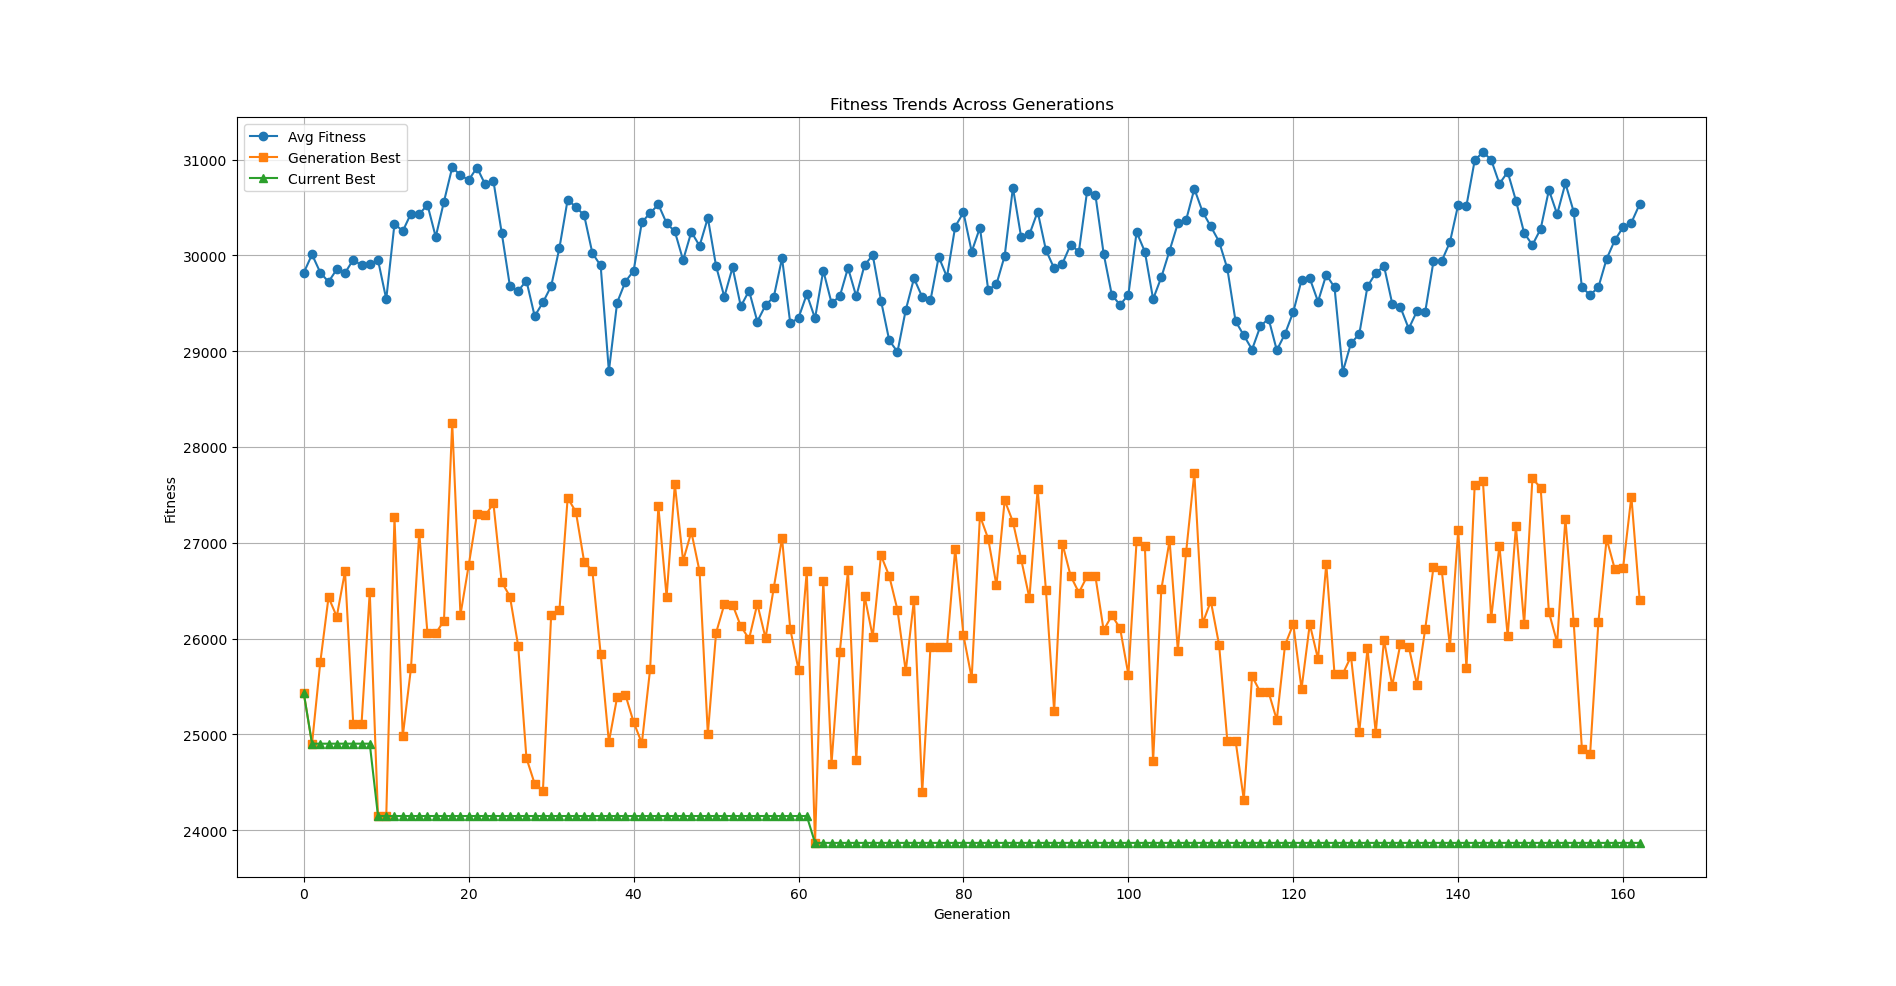
\includegraphics[width=\textwidth]{./images/berlin52_monte_defaults.png}
    \caption{Fitness over 200 generations for \texttt{berlin52.tsp} using Monte Carlo selection }
\end{figure}

As can be seen in the above figure, the algorithm didn't seem to be learning anything and, if anything, fitness seemed to be getting worse over generations.
Probably, the cause of this was that the weighting for Monte Carlo selection was not biased enough in favour of good solutions and against weak solutions, and it just resulted a fairly egalitarian deselection process which destroyed each generation's progress.
Any good solutions found from this process were more as a result of sheer luck than as a result of anything that can be described as learning or evolution.
I tried the same thing with a tournament selection process instead, and got the following results:

\begin{figure}[H]
    \centering
    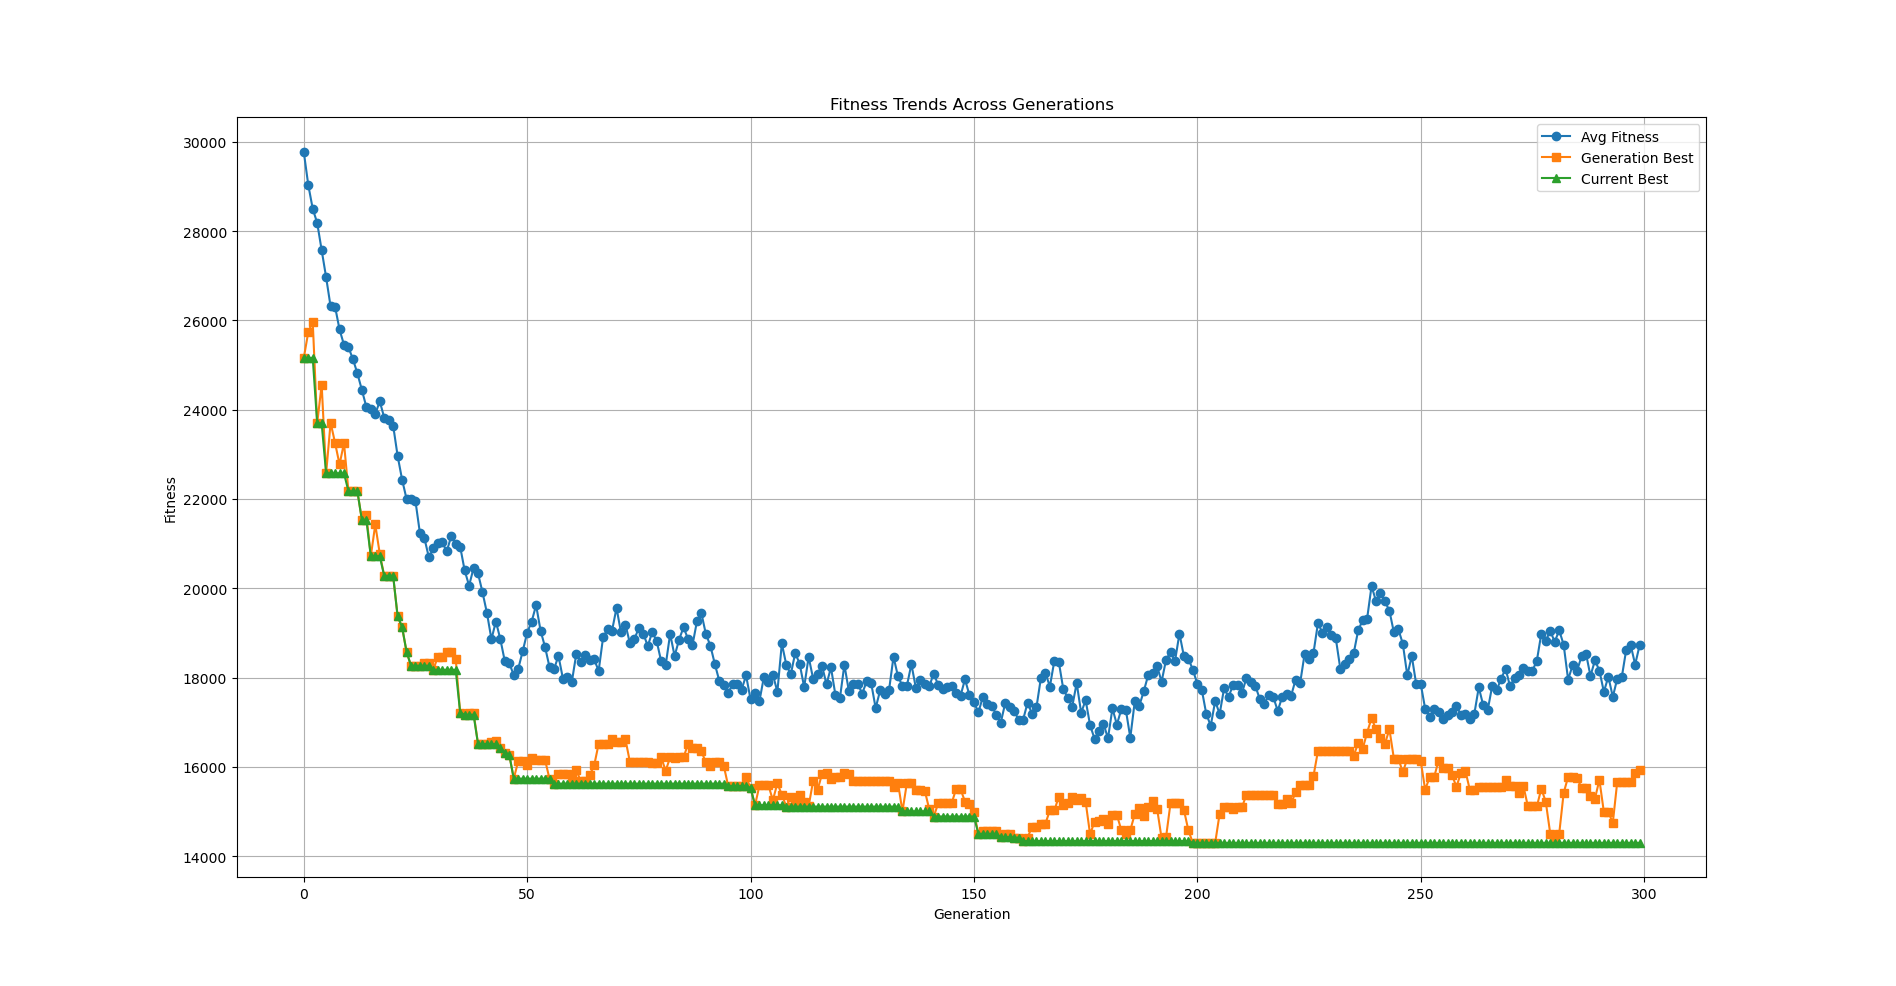
\includegraphics[width=\textwidth]{./images/berlin_52_tourn_defaults.png}
    \caption{Fitness over 200 generations for \texttt{berlin52.tsp} using tournament selection with a tournament size of 3}
\end{figure}

The difference in efficacy was so stark that I immediately abandoned using Monte Carlo selection in favour of tournament selection, although the failure of Monte Carlo selection here was more likely a result of poor implementation than as a result of genuine inappropriateness for the problem.
Tournament selection maintained the diversity I was looking for, giving an opportunity for survival to weaker solutions while maintaining a healthy population of increasingly fit solutions.

\subsubsection{Crossover}
Crossover is performed on the survivors of the selection process using a generalised \texttt{crossover(population, crossover\_rate, number\_to\_replace)} function which randomly alternates between Partially Mapped Crossover (PMX) and Order Crossover (OX), the algorithmic steps for which I took from Wikipedia\supercite{crossover}; while not a scholarly source for a reference, I feel that it's reasonable to use for the algorithmic steps in this case as they evidently produce the desired the results or do not and can be quite easily verified.
\\\\
The PMX operator works as follows:
first, two indices within the two parent solutions are selected at random to serve as crossover points.
If the first crossover point occurs after second in the list, they are swapped.
Then, the sub-sequence from the first parent from the first crossover point to the second is copied directly to the child solution in the same positions.
Then, the second parent is iterated over from the first crossover point to the second crossover point:
for each city $m$ in the second parent that is not yet in the child solution, the city $n$ that occurs in the child at the index at which $m$ occurs in the parent is selected.
The index of $n$ in the second parent is found to create the partial mapping, and $m$ is copied into the child at the index at which $n$ occurs in the second parent, provided that index is empty in the child.
If the index occupied by $n$ in the parent is already occupied by some element $k$ in the child, $m$ is placed in the child at the index at which $k$ occurs in the second parent.
After the genes from the selected sub-sequence in the second parent are all copied into the child, the remaining positions in the child are filled with the genes from the second parent that still have yet to be copied into the child in the order that they appear in the second parent.
This is done by iterating over each index in the second parent, and if the city at that index is not found in the child, it is inserted into the child in the next empty position, until every city is accounted for and every index in the child is filled.
Thus, high-quality sub-sequences that have evolved in the parents have a chance of being preserved in the child, while introducing variance.
The partial mapping allows us to ensure that the child solution remains a valid solution with no duplication of cities.
\\\\
The OX operator works as follows:
like the PMX operator, two crossover points are selected at random and the sub-sequence defined by these crossover points is copied directly into the child.



\section{Experimental Results \& Analysis}
\subsection{Performance Comparison with Known Optimal Solution}
\section{Potential Improvements}

\nocite{*}
\printbibliography

\end{document}
